%        File: MTC.tex
%     Created: Thu Jan 12 02:00 PM 2017 E
% Last Change: Thu Jan 12 02:00 PM 2017 E
%
% arara: pdflatex: {options: "-draftmode"}
% arara: biber
% arara: pdflatex: {options: "-draftmode"}
% arara: pdflatex: {options: "-file-line-error-style"}
\documentclass[Proposal]{subfiles}

\begin{document}
\begin{frame}
  {What are the \textit{ec}s?}
  \begin{block}
    {Two possibilities:}
    \begin{enumerate}
      \item PRO
	\begin{itemize}
	  \item PRO-theory \parencite{chomsky1981lectures,culicover2001control,landau2003movement}
	  \item Standardly assumed
	\end{itemize}
      \item Traces/Copies
	\begin{itemize}
	  \item Movement Theory of Control \parencite{hornstein1999movement,boeckx2003reply,boeckx2006virtues}
	  \item Non-standard
	\end{itemize}
    \end{enumerate}
  \end{block}
\pause
I will assume the Movement Theory of Control.
\end{frame}
\begin{frame}
  {Why MTC?}
  {Theoretical rationale \parencite[see also][]{hornstein2001move}}

  \begin{itemize}
    \item PRO is required by the $\Theta$-criterion
  \end{itemize}
  \ex. Each argument bears one and only one $\Theta$-role, and each $\Theta$-role is assigned to one and only one argument. \parencite[36]{chomsky1981lectures}

\end{frame}
\begin{frame}
  {Why MTC?}
  {Theoretical rationale \parencite[see also][]{hornstein2001move}}
 
  \begin{columns}
    \begin{column}[T]{0.5\textwidth}
      \begin{itemize}
	\item The $\Theta$-criterion follows from the GB model of the grammar
	  \begin{itemize}
	    \item $\Theta$-roles assignment is represented at D-structure.
	    \item Movement operations derive S-structures from D-structures.
	  \end{itemize}
	\item Since arguments are displaced by movement and movement follows $\Theta$-role assignment, movement into $\Theta$-positions is ruled out.
      \end{itemize}
    \end{column}
    \begin{column}[T]{0.5\textwidth}
      {\small
  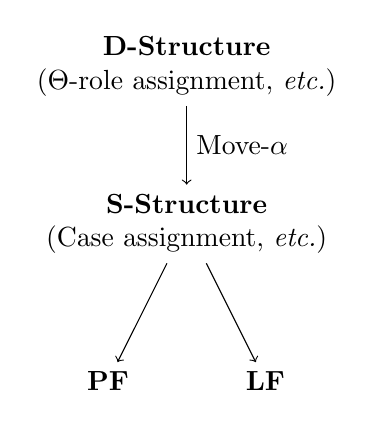
\begin{tikzpicture}
    \node[align=center] (DS) at (0,0){\textbf{D-Structure}\\($\Theta$-role assignment, \textit{etc.})};
    %\node[right=of DS,align=left] (DS stuff) {};
    \node[align=center] (SS) at (0,-2){\textbf{S-Structure}\\(Case assignment, \textit{etc.})};
    \node (LF) at (1,-4) {\textbf{LF}};
    \node (PF) at (-1,-4) {\textbf{PF}};
    \draw[->] (DS) -- (SS)
      node[midway,right] {Move-$\alpha$};
      \draw[->] (SS) -- (LF);
      \draw[->] (SS) -- (PF);
  \end{tikzpicture}}
    \end{column}
  \end{columns}
\end{frame}
\begin{frame}
  {Why MTC?}
  {Theoretical rationale \parencite[see also][]{hornstein2001move}}
  \begin{itemize}
    \item Control only \textit{seems} to be an instance of 1 argument with 2 $\Theta$-roles.
  \end{itemize}
  \ex.* Richard$_i$ wanted [$t_i$ to laugh].

  \begin{itemize}
    \item Instead control involves 1 independent argument and 1 anaphoric argument each with 1 $\Theta$-role.
  \end{itemize}
  \ex. Richard$_i$ wanted [PRO$_i$ to laugh].

\end{frame}
\begin{frame}
  {Why MTC?}
  {Theoretical rationale \parencite[see also][]{hornstein2001move}}

  \begin{itemize}
    \item Minimalist theorizing has dispensed with D- and S-structures.
      \pause
    \item There is no longer a rationale  for the $\Theta$-criterion.
      \pause
    \item There is no longer a rationale for the existence PRO.
      \pause
    \item MTC should be assumed by default.
  \end{itemize}
\end{frame}
\begin{frame}
  {Why MTC?}
  {Methodolgical rationale}

  \begin{itemize}
    \item Movement is reducible to Merge. \parencite{chomsky2004beyond}
    \item Merge is well-defined and well understood.
  \end{itemize}
  \ex. Merge($\alpha, \beta$) = $\left\{ \alpha, \beta \right\}$

  \begin{itemize}
    \item Merge is simple and austere.
  \end{itemize}
\end{frame}
\end{document}


